%%%%%%%%%%%% Attribution %%%%%%%%%%%%
% This template was created by 
% Chuck F. Rocca at WCSU and may be
% copied and used freely for 
% non-commercial purposes.
% 10-17-2021
%%%%%%%%%%%%%%%%%%%%%%%%%%%%%%%%%%%%%

%%%%%%% Start Document Header %%%%%%%
% In creating a new document
% copy and paste the header 
% as is.
%%%%%%%%%%%%%%%%%%%%%%%%%%%%%%%%%%%%%
\documentclass[12pt]{article}

\usepackage{tikz} 
\usepackage{geometry}
\usepackage{listings}
\usepackage{pdfpages}
\usepackage{hyperref}
\usepackage{minted}
\hypersetup{
    colorlinks=true,
    linkcolor=blue,
    filecolor=magenta,      
    urlcolor=cyan,
    pdftitle={Overleaf Example},
    pdfpagemode=FullScreen,
    }

\urlstyle{same}
\geometry{margin=1in}
%%%% Header Information %%%%

%%%% Document Information %%%%
    \title{RME 3111 - Lab 2: Heap}
    \author{
    Course Instructor: Dr. Sejuti Rahman\\
    \\
    Md. Arban Hossain (SH-092-005)\\
    }
    \date{09 Feb 2023}

%%%%%%% End Document Header %%%%%%%


%%%% Begin Document %%%%
% note that the document starts with
% \begin{document} and ends with
% \end{document}
%%%%%%%%%%%%%%%%%%%%%%%%

\begin{document}

%%%% Format Running Header %%%%%

%%%% Insert the Title Information %%%
\maketitle


%%%% Introduction to the General Template %%%%
\subsection*{The A* Algorithm}
The A* algorithm is an informed search algorithm that uses a heuristic function to guide the search. The heuristic function is used to estimate the cost of the path from the current vertex to the destination. It is guaranteed to find the shortest path if the heuristic function is admissible. An admissible heuristic function is one that never overestimates the cost of the path from the current vertex to the destination.

\[ h(n) \leq d(n) \]
\noindent
Here,

$h(n)$ = The heuristic cost of the path from the vertex to destination

$d(n)$ = The actual cost of the path from the vertex to destination


\subsection*{Pen and Paper Simulation}

Consider the following graph. The vertices are labeled with their names and the edges are labeled with their costs. The graph is directed.

\begin{center}
  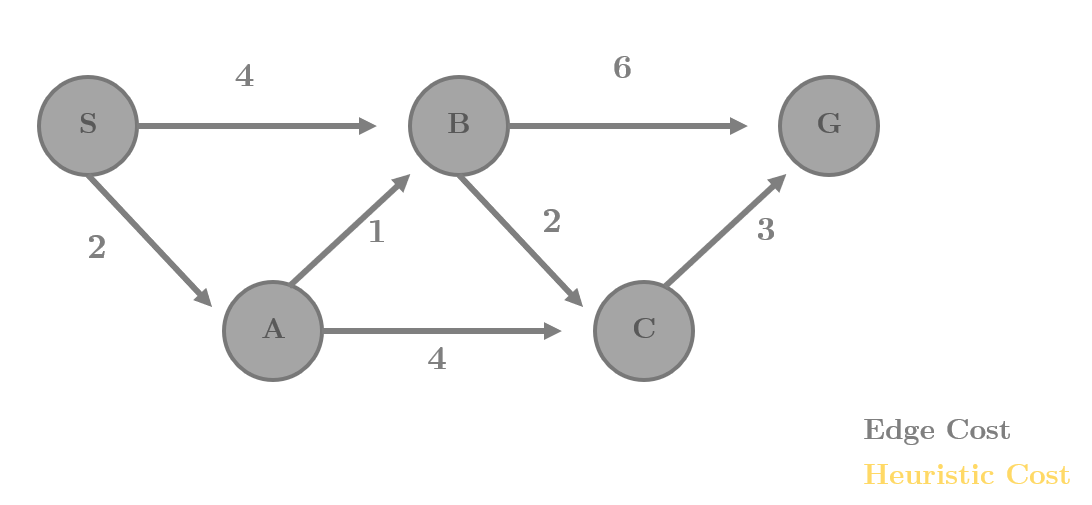
\includegraphics[width=0.9\textwidth]{Graph.png}
\end{center}

\subsection*{Heuristic 1}

For the following set of heuristics, we can simulate the search process manually.

% A table containing 2 columns, one for the vertex name and the other for the heuristic cost.
\begin{center}
  \begin{tabular}{|c|c|}
    \hline
    Vertex & Heuristic Cost\\
    \hline
    S & 8\\
    \hline
    A & 3\\
    \hline
    B & 7\\
    \hline
    C & 2\\
    \hline
    G & 0\\
    \hline
  \end{tabular}
\end{center}

% Add images of heuristic1_Page 1 to 6

\begin{center}
  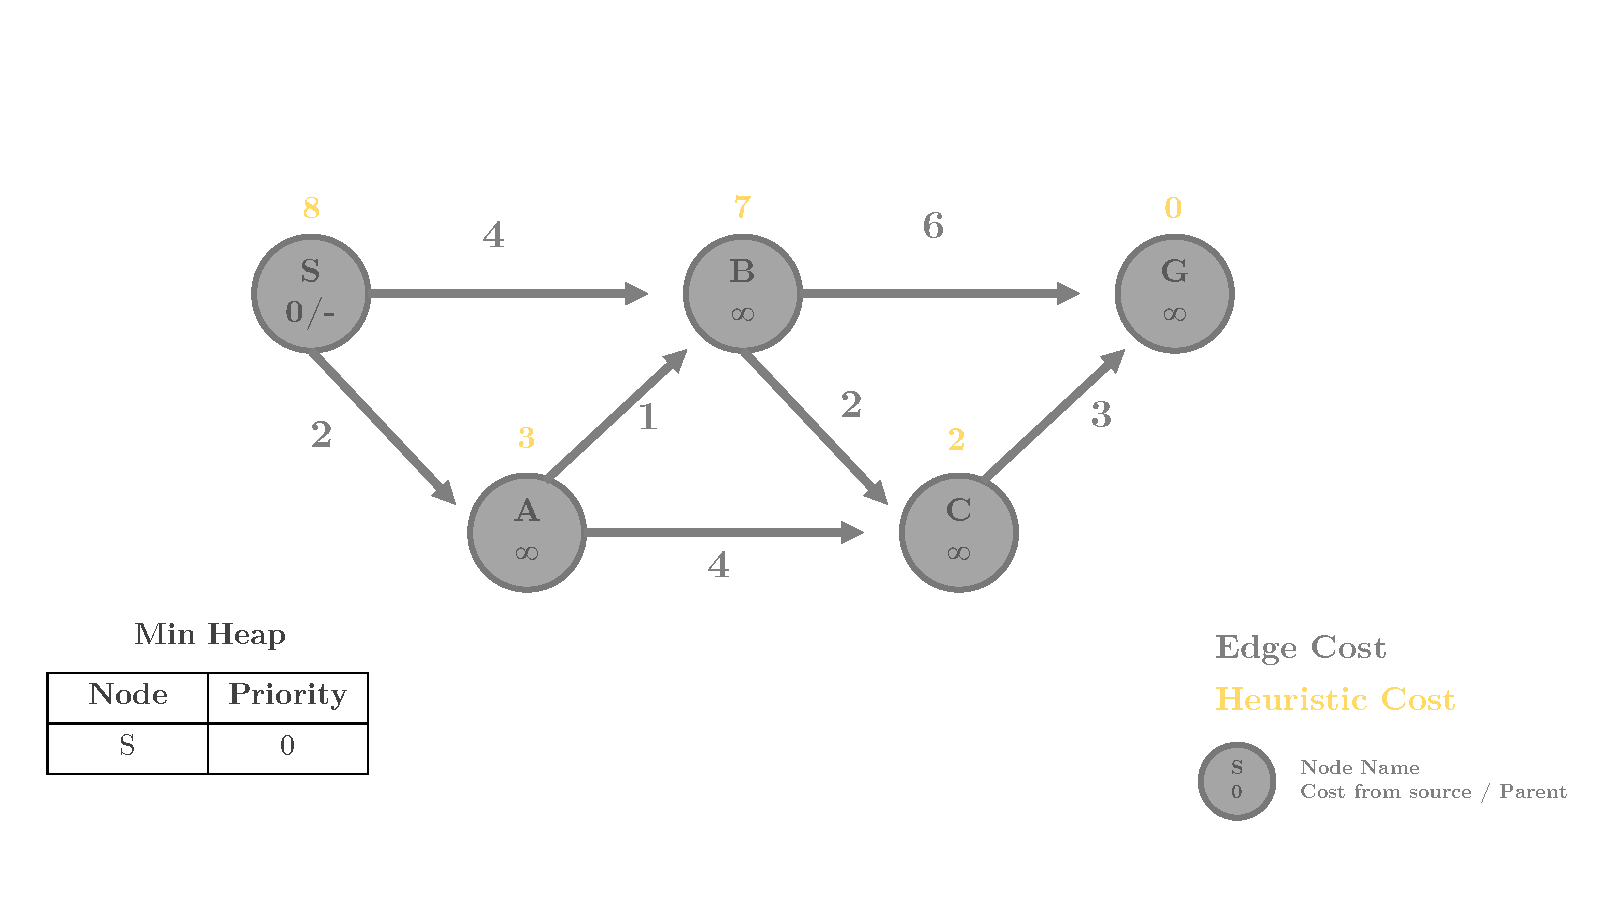
\includegraphics[width=0.9\textwidth]{heuristic1_Page1.png}
\end{center}

\begin{center}
  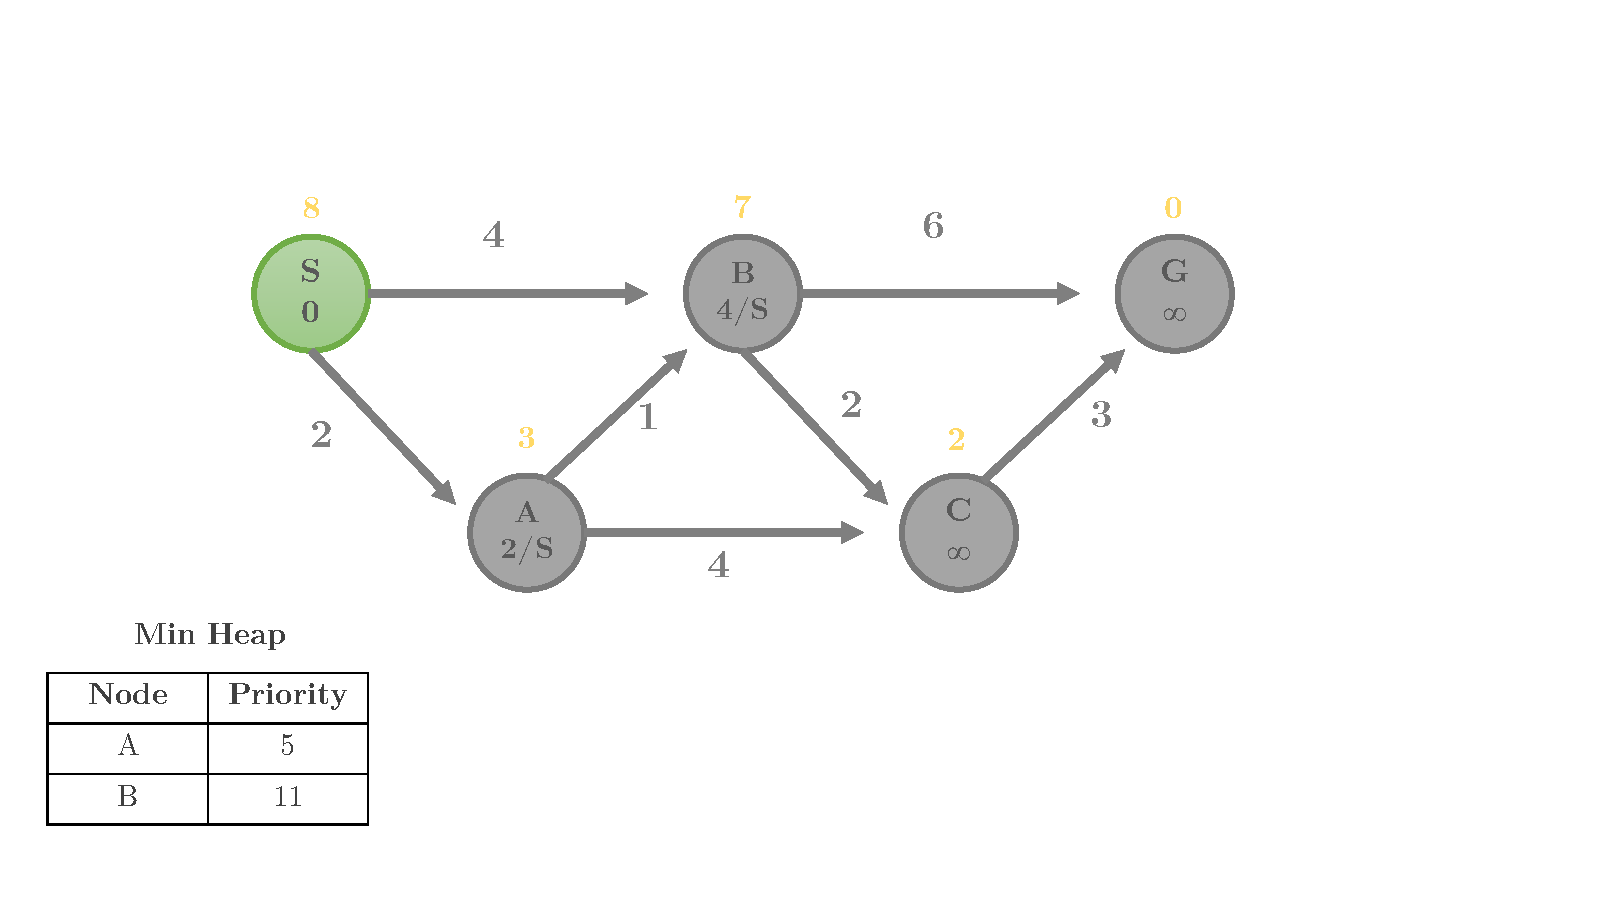
\includegraphics[width=0.9\textwidth]{heuristic1_Page2.png}
\end{center}

\begin{center}
  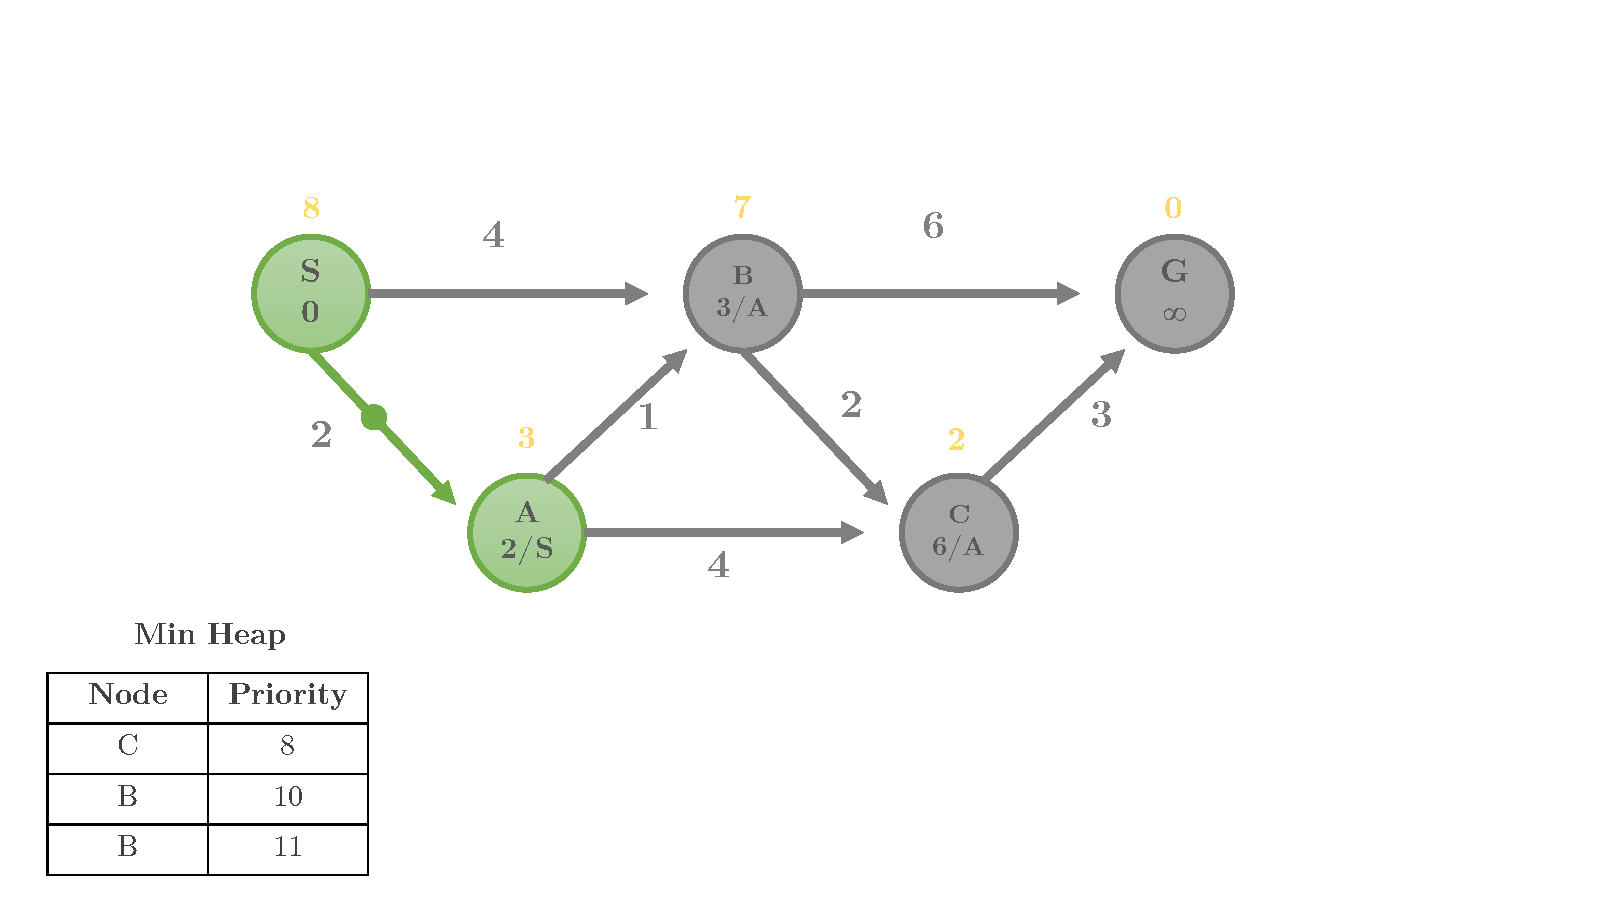
\includegraphics[width=0.9\textwidth]{heuristic1_Page3.png}
\end{center}

\begin{center}
  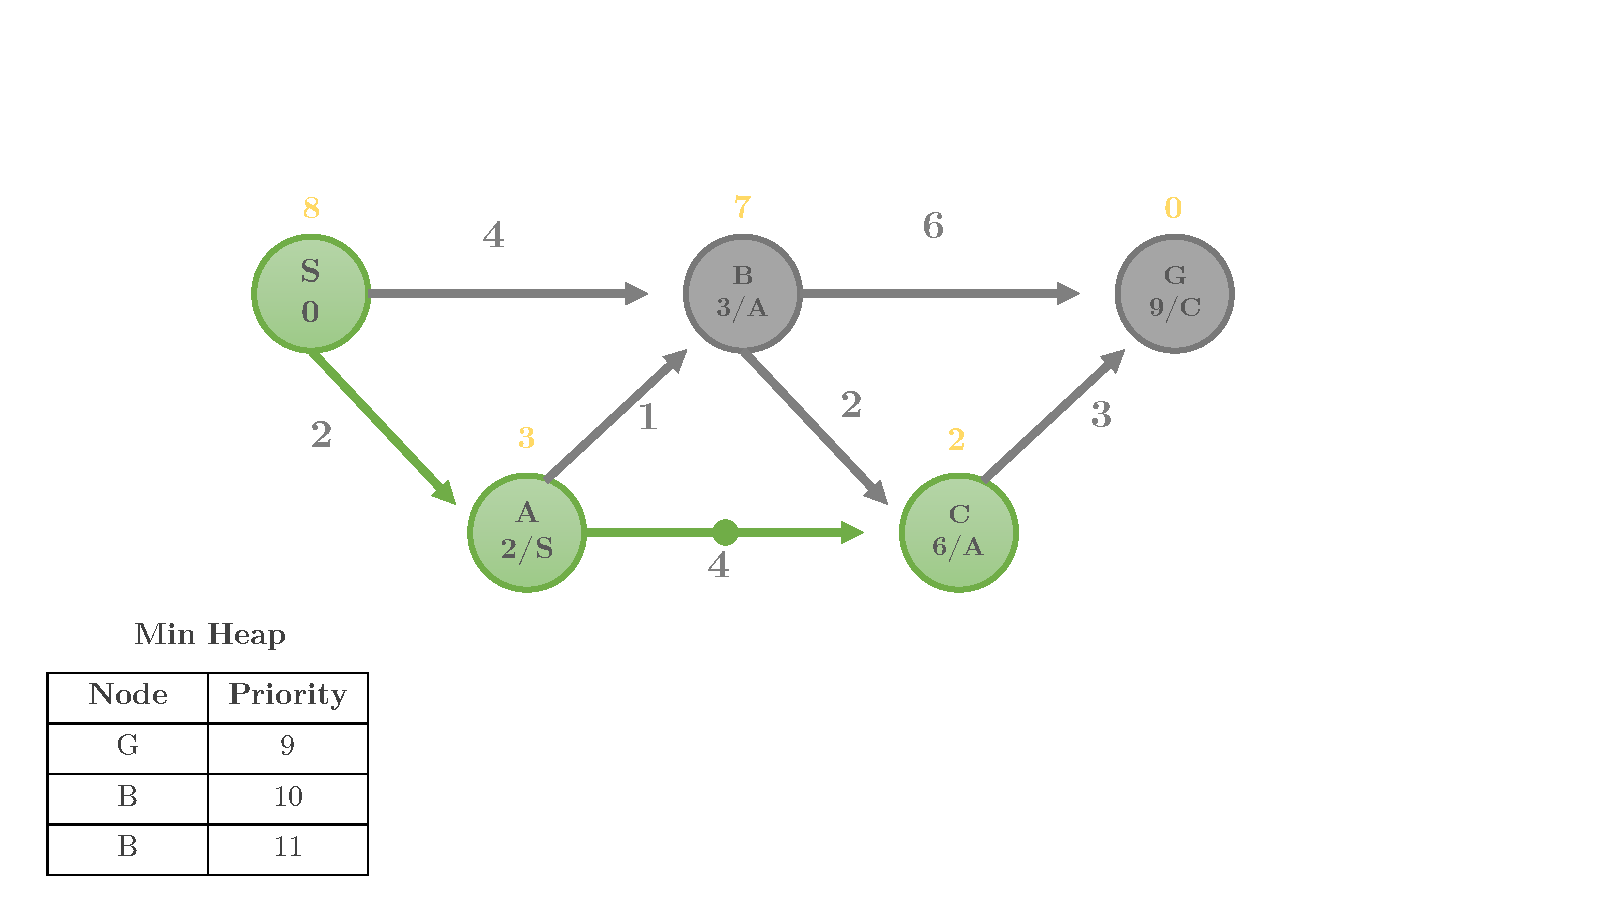
\includegraphics[width=0.9\textwidth]{heuristic1_Page4.png}
\end{center}

\begin{center}
  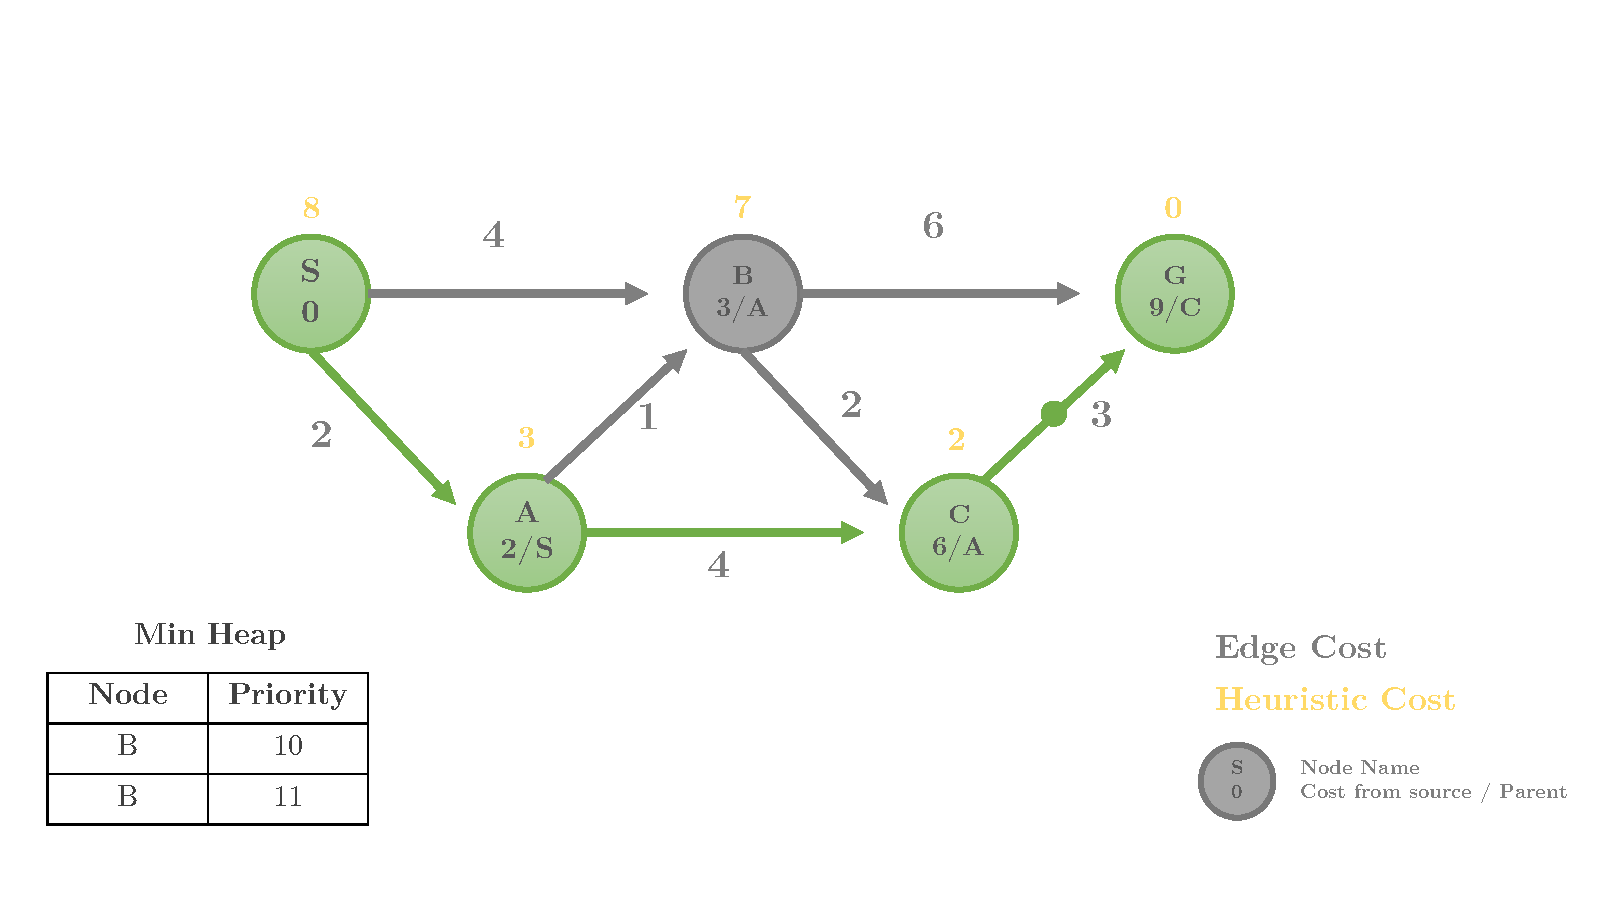
\includegraphics[width=0.9\textwidth]{heuristic1_Page5.png}
\end{center}

\begin{center}
  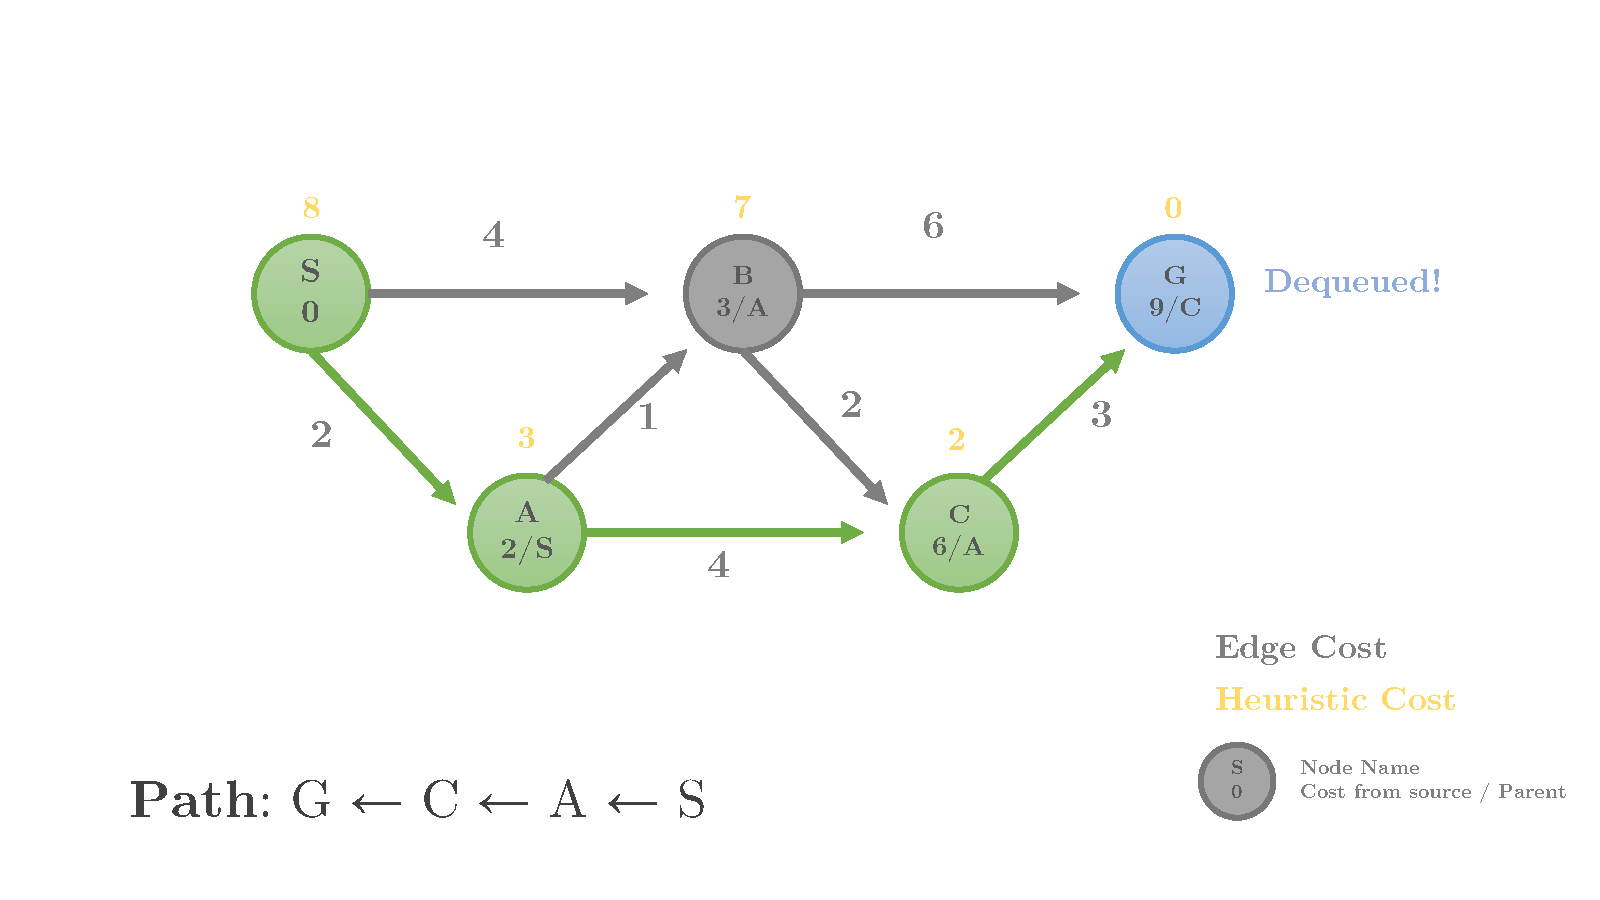
\includegraphics[width=0.9\textwidth]{heuristic1_Page6.png}
\end{center}

Before implementing the code, let's search through the graph manually documenting our process. Use vertex \#2 as our source and vertex \#1 as our destination.

\vspace{5mm} %5mm vertical space

To start the Breadth First Search, push the source vertex into a queue \textbf{Q}. Use a \textit{set} \textbf{Visited} to keep track of the visited vertices. At each iteration of the search, pop an item from the queue, mark it as visited, and check each of its neighboring vertices. We have found our path if one of the neighbors is the destination. Otherwise, push the neighbors into the queue if they have not been visited and resume the process. Terminate the process when we have: (a) reached our destination, or (b) visited all vertices reachable from the 

Before starting the search, the states of \textbf{Q} and \textbf{Visited} are:

\textbf{Q}: 2

\textbf{Visited}: \{\}

\subsubsection*{Iteration 1}
\begin{itemize}
  \item Pop an item (2) from \textbf{Q}. Add it to \textbf{Visited}.
  \item Check its neighbors. In this case, 3 and 0. None of them is the destination. None of them is in \textbf{Visited}.
  \item Push 3 and 0 into \textbf{Q}.
\end{itemize}

\textbf{Q}: 3 0

\textbf{Visited}: \{2\}


\subsubsection*{Iteration 2}
\begin{itemize}
  \item Pop an item (3) from \textbf{Q}. Add it to \textbf{Visited}.
  \item Check its neighbors. In this case, 3. It is not the destination. It is in \textbf{Visited}. So do nothing.
\end{itemize}

\textbf{Q}: 0

\textbf{Visited}: \{2, 3\}



\subsubsection*{Iteration 3}
\begin{itemize}
  \item Pop an item (0) from \textbf{Q}. Add it to \textbf{Visited}.
  \item Check its neighbors. In this case, 2 and 1. One of them (1) is the destination. Add it to \textbf{Visited}. We can now terminate our search and return a \textbf{True} value.
\end{itemize}

\textbf{Q}: Empty

\textbf{Visited}: \{2, 3, 0, 1\}

\pagebreak
\section*{Part B}

\subsection*{Source Code}
Python3 source code for the problem follows.

\begin{minted}
[
baselinestretch=1.2,
fontsize=\footnotesize,
]{python}
### Lab1.py

class Node:

  def __init__(self, elem):
    self.value = elem
    self.next = None

class Queue:

  def __init__(self):
    self.head = None
    self.tail = None

  # O(1)
  def is_empty(self):
    return self.head == None
  
  # O(1)
  def enqueue(self, elem):
    node = Node(elem)
    if self.head == None:
      self.head = node
      self.tail = node
    else:
      self.tail.next = node
      self.tail = node
  
  # O(1)
  def dequeue(self):
    if self.head == None: return None
    else:
      node = self.head
      self.head = self.head.next
      return node.value

class Vertex:

  def __init__(self, name, value=None):
    self.value = value
    self.name = name

# Space: O(V) for vertices. O(E) for edges. Total O(V+E)
class Graph:

  def __init__(self):
    self.adjacency_list = {}
    self.vertices = {}
  
  def add_directed_edge(self, v1, v2):
    # add vertex in vertices if not already there
    if v1.name not in self.vertices:
      self.vertices[v1.name] = v1
    if v2.name not in self.vertices:
      self.vertices[v2.name] = v2
    
    # add v2 in v1's adjacency list
    if v1.name in self.adjacency_list:
      self.adjacency_list[v1.name].append(v2.name)
    else:
      self.adjacency_list[v1.name] = [v2.name]
    
    if v2.name not in self.adjacency_list:
      self.adjacency_list[v2.name] = []
  
  # Time: O(V+E)
  # Space: O(V)
  def path_exists_bfs(self, v1, v2):
    queue = Queue()
    queue.enqueue(v1)
    visited = set()
    while not queue.is_empty():
      current = queue.dequeue()
      if current not in visited:
        visited.add(current)
        if current == v2:
          return True
        for neighbor in self.adjacency_list[current]:
          if neighbor == v2:
            return True
          queue.enqueue(neighbor)
    return False



if __name__ == "__main__":
  no_of_vertices, edges, source = map(int, input().split())
  
  graph = Graph()

  for _ in range(edges):
    v1, v2 = [Vertex(x) for x in input().split()]
    graph.add_directed_edge(v1, v2)
  
  for _ in range(int(input())):
    v1, v2 = [x for x in input().split()]
    print(graph.path_exists_bfs(v1, v2))
\end{minted}
\pagebreak
\subsection*{Output}
Using the provided input file, the output of the program was:
\

\subsection*{Complexity Analysis}
\subsubsection*{Time Complexity}
The function \textbf{path\_exists\_bfs()} iterates over all the vertices at most once. For each vertex, it iterates over all the edges it is connected to. During each iteration, it takes \textbf{O(1)} time for the \textit{push} and \textit{pop} operations of the queue. Looking up an item in a Python \textit{set} also takes \textbf{O(1)} time. Considering the graph has \textbf{V} vertices and \textbf{E} edges, in the worst case it will take \textbf{O(V+E)} time to finish the search.

\subsubsection*{Space Complexity}
The adjacency list is implemented using a Python dictionary. During each iteration, all neighboring vertices of the current vertex are present in the queue. In the worst case, this number can be equal to the number of total vertices in the graph. So it takes \textbf{O(V)} space.

\subsection*{Links}
The source files can be found at \href{https://github.com/arbanhossain/RME_31x1/tree/main/Labs}{github.com/arbanhossain/RME\_31x1}.

\end{document}
